\documentclass{MScthesisITEM}

% this package is just to generate text for demo-purposes
%\usepackage{blindtext}
\usepackage{float}

\usepackage{hyperref}
%\usepackage[section]{minted}
%\usepackage{aeguill}
%\usepackage{placeins}
%\usepackage[T1]{fontenc}
%\usepackage{tabulary}

\showboxdepth=5
\showboxbreadth=5

\title{Learning Modeling Languages Using\newlinetitle Strategies from Gaming} % The title of your assignement; NB use \newlinetitle to start a newline
\author{\O yvin Richardsen} % Your firstname and lastname
\professor{Frank Alexander Kraemer, ITEM NTNU} % Affiliation = ITEM for instance
\supervisor{Frank Alexander Kraemer, ITEM NTNU}

%% Uncomment the following in case you want subfigures; note that there will be a warning for the caption package
%\let\subcaption\undefined
%\let\subfloat\undefined
%\usepackage[bf]{caption}
%\usepackage{subcaption}
%\captionsetup{compatibility=false}


\DeclareGraphicsExtensions{.pdf,.jpg,.png}
\graphicspath{{./img/}}

\loadglsentries{glossary}
\makeglossaries

\begin{document}
\selectlanguage{english}
\pagenumbering{roman}
\pagestyle{plain}

%% Only for the project
\titleITEM

%% Only for the master's thesis; for the project report the description is taken from It's Learning and added by the department
\selectlanguage{english} % Change to 'norsk' if you are writing in Norwegian
\chapter*{Problem Description}
When learning to use a software modeling language, people are usually directed towards the language's documentation, or ``language tutorials'' in the form of a set of instructions required to get started with the language. Most of the information about the language is generally delivered early in the process, requiring the developer to either understand (and remember) a lot of concepts at once, or to go back and search for the information when it's needed.

\noindent
On the contrary, many computer games come with no instructions at all, but rather start by guiding the player through a set of training levels. Each level introduces a new element, concept or strategy, and sometimes let the player experiment with the new concepts to solve more advanced problems.

\noindent
In this thesis, it will be examined to which degree this approach can be used for introducing and learning a new modeling language. Methods for creating more immersive tutorial experiences with required information delivered in-context will be explored and tested, using UML Activities and the Reactive Blocks tool as an example. The thesis will also explore whether the context of the tutorial matters, and if there are possible advantages gained by designing the tutorial experience itself as a game.

\noindent
\textbf{Assignment given:} \emph{Learning Modeling Languages Using Strategies From Gaming} \\
\textbf{Supervisor:} Frank Alexander Kraemer
\cleardoublepage

%% There must be an abstract in English, even though the main text is in Norwegian
%\selectlanguage{english}
%\chapter*{Abstract}

%\cleardoublepage

%% Only for the master's thesis; if the main text is in English and you can write Norwegian, there must be an abstract in Norwegian as well.A
%\selectlanguage{norsk}
%Abstract nor: TODO
%\cleardoublepage

\selectlanguage{english}% Change to 'norsk' if you are writing in Norwegian

\chapter*{Preface}

This thesis is submitted as the concluding part of my Master of Science degree in Communication Technology at the \gls{ntnu}. The supervisor for this thesis has been Associate Professor Frank A. Kraemer, and I would like to thank him for his help and guidance. I would also like to thank the people who helped me with the testing of my work.

\noindent
Trondheim, June 2014 \\
{\O}yvin Richardsen
\cleardoublepage

% similarly you may add a separate acknowledgments page

\tableofcontents*
\cleardoublepage

%% include if relevant
\listoffigures
\cleardoublepage

%% include if relevant
%\listoftables
%\cleardoublepage

%% include if relevant
%\listofalgorithms
%\addcontentsline{toc}{chapter}{List of Algorithms}
%\cleardoublepage


%% include if relevant
%\printglossary[title=List of Symbols, style=long]
%\cleardoublepage
%\glsaddall[]

%% include if relevant
%\printglossary[title=List of Acronyms,type=\acronymtype] % prints just the list of acronyms
%\cleardoublepage

\pagenumbering{arabic}
\pagestyle{ruled}
\chapter{Introduction}
\label{ch:intro}

\section{Problem Definition and Scope}
\label{sec:scope}


\subsection{Organization of the Report}
\cleardoublepage
\chapter{Background}
\label{ch:background}
This chapter contains the background material that serves as the basis for this thesis. The following sections are a mix of summarizations of other people's work, and some gathering and analysis of information done by me.


\section{Software Modeling and Modeling Languages}
\label{sec:software_modeling}
In the world of software development, potential problems and challenges that may arise when developing a product are plentiful.


\subsection{The Purpose of Software Modeling}


\subsection{Modeling Languages}


\subsection{Automatic Code Generation}


\section{Tutorials}
\label{sec:tutorials}
``A tutorial is a method of transferring knowledge and may be used as a part of a learning process. More interactive and specific than a book or a lecture, a tutorial seeks to teach by example and supply the information to complete a certain task.''~\cite{wiki:tutorial}

\noindent
Tutorials are often used to teach and introduce new concepts and topics to users who previously have little or no experience with it. Tutorials may be designed for learning a vast range of topics and concepts, such as:
\begin{itemize}
	\item Programming, or using specific programming or modeling languages.\footnote{\url{http://docs.oracle.com/javase/tutorial/}, \url{http://www.tutorialspoint.com/uml/}}
	\item Spoken languages.\footnote{\url{http://ielanguages.com/}}
	\item Software products.\footnote{\url{http://www.photoshoptutorials.ws/category/photoshop-tutorials/}}
	\item Video games (such tutorials are usually presented inside the game itself)
	\item Real-life skills, like photography.\footnote{\url{http://photography.tutsplus.com/}}
	\item Human sciences.\footnote{\url{http://anthro.palomar.edu/tutorials/}}
\end{itemize}

\noindent
The above list is in no way exhaustive, but meant to offer some examples of the numerous and diverse topics that may be introduced with the help of a tutorial.

\noindent
Additionally, tutorials come in many forms. The most common form of tutorial is likely the text-based tutorial, often supplemented by illustrations and pictures, but tutorials also come in the form of videos, animations, audio, or in the case of many video games, an interactive experience combining any or all of these.

\subsection{The Structure of a Tutorial}
\label{sec:tutorial_structure}
Tutorials for different types of topics are generally structured in a way the author believes will provide a good introduction for the given topic, starting with the necessary basic information, and then building on this to learn more advanced concepts. Depending on both the topic and the author, this may result in very different structures.

\noindent
Looking at some of the examples from Sect.~\ref{sec:tutorials}, we see that while the Java tutorials provide stepwise instructions for reaching a specific goal, the spoken language tutorials serve as more of a lookup reference for the most basic concepts within the language. The spoken language tutorials are actually in some ways similar to the separate Java API documentation.\footnote{\url{http://docs.oracle.com/javase/8/docs/api/index.html}}

\noindent
While there are differences in how tutorials for various topics are made, we may infer some general patterns and elements present in a wide range of different tutorials.

\begin{itemize}
	\item Basic and/or advanced information about the topic, depending on the scope of the tutorial. Often presented in a stepwise manner, starting from the most basic and moving on to the more advanced.
	\item Examples on how to use the information provided in specific cases or contexts.
	\item Exercises where the reader must try to use the concepts introduced in a specific context.
	\item Illustrations, figures, or animations, providing the reader with additional examples, information about concepts, or desired results from exercises.
	\item Some kind of motivation for learning about the topic, often as part the tutorial introduction.
\end{itemize}

\noindent
How these patterns and elements are presented depends on the form of the tutorial.

\subsection{The Characteristics of a Tutorial}
\label{sec:tutorial_characteristics}


\subsection{What Makes a Tutorial Good?}


\section{Tutorials for Programming and Software Modeling}
\label{sec:programming_tutorials}
In order to teach potential users to use a specific programming language, paradigm, protocol or modeling language (from now on referred to simply as a \emph{topic}), various additional tools or sources of information may be provided. Generally, some form of formal documentation or specification of the language or protocol is considered mandatory, and serves as the \emph{definitive} source of information. Additionally, various tutorials and exercises are often created in order to provide a better introduction to the topic, decreasing the threshold for learning this topic.

\subsection{Documentation}
While a topic's documentation often serves as its primary source of information, such formal documents are not necessarily the best source of information when \emph{learning} about the given topic. Often it is not intended as a learning resource, but rather as a formal reference for users already familiar with the topic. In the documentation, the topic is generally presented in a structured way with respect to its various aspects, so that it is easy for someone already familiar with the topic to find the required information.

\noindent
A good example of this is the \gls{uml} specification.\footnote{\url{http://www.omg.org/spec/UML/2.4.1/}} While the specification offers detailed information about every aspect of \gls{uml} in a way that suits an experienced user, it is likely confusing and not particularly helpful for a user with no previous experience or knowledge about \gls{uml}. Using this specification as a starting point for learning \gls{uml} is likely to require a lot of effort from the user. In the worst case, the user may not even learn all the concepts properly, despite the provided information being very specific and accurate.

\noindent
More importantly, the user may not learn how to properly apply the learned concepts to a given situation. In many cases, 


\subsection{Advantages and Challenges}




\section{Game-based learning}
\label{sec:game_based_learning}

\subsection{Gamification}


\subsection{Learning Inside the Game}


\subsection{Applying Acquired Knowledge and Skills in the Game}




\section{Tutorials in Games}
\label{sec:tutorials_in_games}


\subsection{Purpose}

\subsection{Tutorial Characteristics and Their Importance}

presence, context-sensitivity, freedom, availability of help-on-demand





\cleardoublepage
\chapter{Analysis of Related Work}
\label{ch:related_work}
This chapter outlines previous work by other researchers that is relevant to this thesis, supplementing the background information provided in Ch.~\ref{ch:background}. A lot of work and research has been and is being done in the field of learning with games and game-like approaches, but for practical reasons (there is a lot of material) this chapter only summarizes what I've found to be most relevant. This primarily includes work on tutorial design and teaching computer-related tasks through games, but some other work is also included to add perspective.

\section{Tutorial Design}
\label{sec:tutorial_design_related}
Tutorials, as described in Sect.~\ref{sec:tutorials}, are widely used to teach users how to work with software products, among other things. With the tutorial, the creators aim to teach users how to perform various tasks with their tool, preferably in a \textbf{quick}, \textbf{intuitive}, \textbf{memorable}, and \textbf{error-free} way. Unfortunately, not all tutorial designs succeed in fulfilling all of these goals, but many efforts have been made to explore different approaches and improve on the standard tutorial design. Some of these are briefly described in the following sections.

\subsection{Stencils-Based Tutorials}
\label{sec:stencils}
The authors of the paper \emph{Stencils-Based Tutorials: Design and Evaluation}~\cite{kelleher:stencils} identify some problems with traditional tutorials: users may miss steps or perform actions that were not intended, and it is often difficult to find the components described in the tutorial.

\noindent
In their work, the authors introduce \emph{Stencils}, which is an alternative way of presenting a tutorial by adding a translucent colored interface layer on top of the original \gls{ui}, with holes highlighting the relevant elements, as seen in Fig.~\ref{fig:stencils}. Additionally, tutorial information is displayed on this layer in the form of sticky notes.

\begin{figure}[htp]
	\centering
	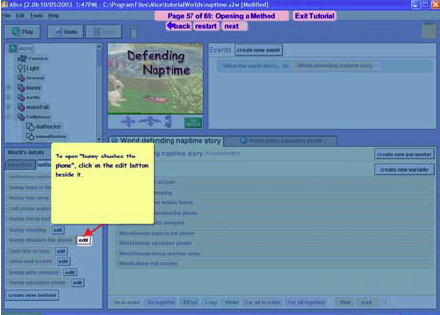
\includegraphics[width=0.8\textwidth]{stencils}
	\caption[\emph{Stencils} example]{An example of highlighting relevant \gls{ui} elements with \emph{Stencils} through holes in the colored layer. Tutorial information is added with the yellow sticky note. \emph{Image source:~\cite{kelleher:stencils}}}
	\label{fig:stencils}
\end{figure}

\noindent
With the results of a user study, the authors show that with a \emph{Stencils}-based tutorial, users were able to complete tutorials faster, with fewer errors and less human assistance. They also note that their tutorial approach can likely be improved by decreasing the level of assistance depending on the users familiarity with the system. A need for tutorial tasks that are directly relevant to the users, as opposed to ``artificial'' tutorial exercises, is also mentioned.


\subsection{DocWizards}
\label{sec:docwizards}
The authors of the paper \emph{DocWizards: A System for Authoring Follow-me Documentation Wizards}~\cite{bergman:docwizards} identify that there are some problems with teaching people to use software (\emph{computer-based procedures}) through documentation alone. Users must find \gls{ui} elements based on documentation descriptions on their own, understand and handle conditional branches, and at the same time keep track of where they are in the process.

\noindent
In their work, they propose the use of a tutorial-like documentation process called \emph{follow-me documentation wizards}, an approach that combines the advantages of conventional wizards and documentation. With their approach, processes are automatically captured from demonstrations made by expert users, and made available to new users in the form of highlighting both text from the documentation (see Fig.~\ref{fig:docwizards}) as well as UI elements for each step.

\begin{figure}[htp]
	\centering
	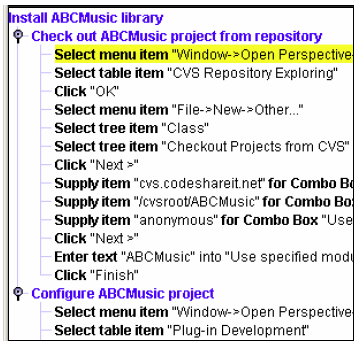
\includegraphics[width=0.6\textwidth]{docwizards}
	\caption[\emph{DocWizards} example]{An example of stepwise instructions in \emph{DocWizards}. The current step is highlighted in yellow. \emph{Image source:~\cite{bergman:docwizards}}}
	\label{fig:docwizards}
\end{figure}

\noindent
TODO: rewrite
Finally, a user study is conducted by the authors to evaluate their system, yielding positive results. The usefulness of the \emph{DocWizards} approach has also been verified in a separate study~\cite{gweon:evaluating_docwizards}.

\subsection{Graphstract}
\label{sec:graphstract}
The authors of the paper \emph{Graphstract: Minimal Graphical Help for Computers}~\cite{huang:graphstract} identify problems with the commonly used approach of providing only a textual explanations in software tutorials and help. Users are unlikely to read these explanations carefully enough, if at all. Simply adding screenshots of the \gls{ui} is not an adequate solution, since these usually add far more information than necessary, and thus increase the perceived size and complexity of the explanation. Problems with animation and video are also identified, such as making it difficult for the user to move at their own pace.

\noindent
Instead of relying on text-only descriptions or simple screenshots, the authors propose the use of graphical help in the form of partial screenshots, combined to show a complete sequence of actions required to perform a task (see Fig.~\ref{fig:graphstract}). This approach provides graphical help directly mapped to the \gls{ui}, without adding a lot of extra information. Additionally, the whole sequence is presented in a small space, making it easy to get an overview.

\begin{figure}[htp]
	\centering
	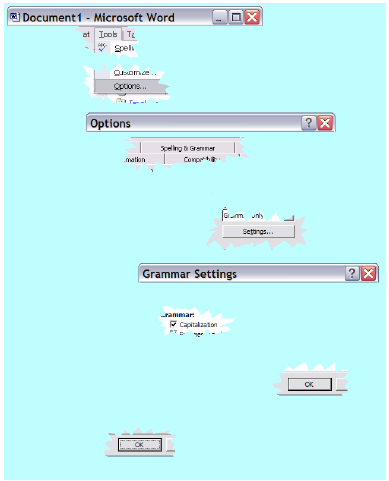
\includegraphics[width=0.7\textwidth]{graphstract}
	\caption[\emph{Graphstract} example]{An example of stepwise instructions in \emph{Graphstract} in the form of screenshot snippets, showing the steps required to toggle auto-capitalization in Microsoft Word. \emph{Image source:~\cite{huang:graphstract}}}
	\label{fig:graphstract}
\end{figure}

\noindent
Three iterations of user studies on a prototype is conducted by the authors, showing that \emph{Graphstract} performs better than conventional approaches overall, if not in all cases. They also conclude that adding text to the images is useful in many situations, despite their approach relying on graphical help only.

\subsection{Photo Tutorials}
\label{sec:photo_tutorials}
The authors of the paper \emph{Generating Photo Manipulation Tutorials by Demonstration}~\cite{grabler:photo_tutorials} argue the use of static visual tutorials (stepwise text-based tutorials accompanied by graphics) over video-tutorials for image processing software.

\noindent
In their work, the authors design a system for auto-generating static visual tutorials for a specific software product. These tutorials provide stepwise instructions with screenshots for completing a particular task, and additionally highlight the parts of the screenshots that are relevant to this task, as seen in Fig~\ref{fig:photo_tutorials}. This is combined with macros for automatic image labeling, to identify important regions of the particular image the user is working with.

\begin{figure}[htp]
	\centering
	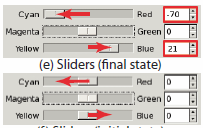
\includegraphics[width=0.5\textwidth]{photo_tutorials}
	\caption[\emph{Photo Tutorials} example]{An example of highlighting relevant \gls{ui} elements in a screenshot with \emph{Photo Tutorials}. \emph{Image source:~\cite{grabler:photo_tutorials}}}
	\label{fig:photo_tutorials}
\end{figure}

\noindent
Through a user study, the authors verify the effectiveness of their tutorials by observing that users perform significantly better and make less errors compared to tutorials based on text and video. However, some problem areas are identified: better tutorials can be created by providing feedback to users as they are performing the steps of the tutorial.

\subsection{Toolclips}
\label{sec:toolclips}
The authors of the paper \emph{ToolClips: An Investigation of Contextual
Video Assistance for Functionality Understanding}~\cite{grossman:toolclips} explore the \emph{learnability} of software products, more specifically relating to the concept of \emph{understanding} how to properly use functionality (see~\cite{grossman:software_learnability}). They identify problems with existing approaches based on both text and videos, where information is provided outside the context of the \gls{ui} in question. The authors also assess that regular tooltips, which provide the user with a short in-context description of what a \gls{ui} element does, do not provide a sufficient level of detail for complex tools.

\noindent
Attempting to provide the best of several worlds, the authors suggest their \emph{ToolClips} approach, enhancing regular tooltips with additional documentation and video content, in a more context-sensitive manner, as seen in Fig.~\ref{fig:toolclips}.

\begin{figure}[htp]
	\centering
	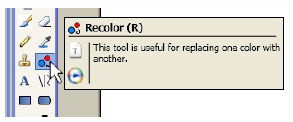
\includegraphics[width=0.7\textwidth]{toolclips}
	\caption[\emph{ToolClips} example]{An example of a \emph{ToolClip}, appearing as a regular tooltip, but with buttons allowing access to additional media. \emph{Image source:~\cite{grossman:toolclips}}}
	\label{fig:toolclips}
\end{figure}

\noindent
Through the results of two user studies, the authors show that the \emph{ToolClips} approach significantly improves users' understanding of how to use elements, and additionally has a positive impact on retention of this understanding, for applications that are \emph{highly graphical}.

\subsection{A Summary of Good Practices for Tutorials}
\label{sec:good_practices_tutorials}
The previous sections in this chapter, as well as Sect.~\ref{sec:tutorials}, describe various research efforts on the creation of good tutorials and introductions for computer-based procedures. Different aspects of the learning process are considered, and it is apparent that there are many ways to succeed. In this section, I attempt to summarize the various aspects that should be considered when making a tutorial for a computer-based procedure.

\paragraph{Interactivity and Active Learning} The most important aspect of a good tutorial is likely that it should be interactive. Active learning is one of Chickering and Gamson's \emph{seven principles of learning}~\cite{chickering:seven_principles}, in addition to being recommended for tutorial design by various other sources~\cite{bowerman:tutorial_design, aberson:tutorial_evaluation}. A common way of making a tutorial interactive is to provide exercises the user must complete.

\paragraph{Feedback} If a user is presented with tasks and exercises during the tutorial, it should also be possible to see the results of these exercises, and if applicable, check if the results are correct~\cite{chickering:seven_principles}. The feedback should also give the user some indication of the user's performance compared to the learning objectives~\cite{bowerman:tutorial_design}.

\paragraph{Motivation} It is important for users to know not only why they should learn the processes described in the tutorial (i.e. how these processes are useful to them), but also why they should complete more advanced tutorials on the subject that may optimize their work~\cite{grossman:software_learnability}. Users should also be informed of the scope of the tutorial, and what they are supposed to learn~\cite{bowerman:tutorial_design}.

\paragraph{Reasonable Teaching Order} If a tutorial teaches multiple concepts, a reasonable teaching order should be established, particularly if these concepts build on each other~\cite{bowerman:tutorial_design}. When deciding on a starting point, user' background must also be considered.

\paragraph{Context-sensitivity of Information} All new information presented in the tutorial should be provided at the point where it is actually needed, as opposed to being presented in an introduction part before the tutorial starts~\cite{andersen:tutorials_impact}.

\paragraph{Visual Mapping of UI Elements} If \gls{ui} elements are referenced in the textual part of a tutorial, it should be easy to map these references to the actual \gls{ui}. This can be done by adding (partial) screenshots of the \gls{ui}~\cite{huang:graphstract}, or highlighting the elements that are relevant for the current step~\cite{kelleher:stencils, bergman:docwizards, grabler:photo_tutorials}.

\paragraph{Multimedia Content} A tutorial that consists of text alone is rarely adequate, and can be improved by adding multimedia content such as images, sound, or video~\cite{grossman:software_learnability}. This kind of multimedia information content can also be present in the application itself, providing the user with more resources when help is needed~\cite{grossman:toolclips}. Animations can also be advantageous, but should be used only where natural, for example to describe events in time~\cite{morrison:animation}.

\paragraph{Help-on-demand} While the user generally shouldn't have to read through too much text before starting the interactive part of the tutorial, additional information resources should be available for when the user gets stuck, or for other reasons needs to know more about a specific topic~\cite{andersen:tutorials_impact, grossman:toolclips}.

\paragraph{Relevant Tasks} When a tutorial contains tasks and exercises, these should be as relevant as possible to the user, as opposed to fictional tasks created only for learning purposes~\cite{kelleher:stencils}.

\paragraph{High Expectations} Users should be presented with high expectations from the beginning, so that they are prepared to make an effort in understanding the concepts taught by the tutorial~\cite{chickering:seven_principles}.

\paragraph{Address Misconceptions} If common misconceptions exist within the topic that is being taught, the tutorial should do its best to address these misconceptions, preferably before they even have a chance to form~\cite{aberson:tutorial_evaluation}.

\paragraph{Multiple Perspectives} Generally, we want the user to actually think reflectively about the topic being taught, and not just passively absorb the facts. One way of doing this is by offering multiple perspectives of various concepts~\cite{aberson:tutorial_evaluation}.

\paragraph{Freedom} When introducing something like a game or a software product through a tutorial, we have to consider the amount of freedom users are given in the tutorial. There are issues in both allowing users complete freedom to explore, and restricting them to a single path~\cite{andersen:tutorials_impact, bonawitz:double_edged_pedagogy}. The optimal solution likely lies somewhere in between, by for example offering \emph{directed exploration}~\cite{esper:codespells}. 

\section{Learning With Games}
\label{sec:learning_with_games}
Most video games require the player to learn something in order to complete the game, whether it is difficult concepts like solving obscure puzzles, or simply the controls of the game. In some cases, games are even used to teach concepts for educational purposes, such as programming. In other cases, games even teach players valuable real-life skills without being deliberately designed to do so. The following sections briefly describe some of the efforts previously made in the field of educational games.

\subsection{Karel the Robot}
\label{sec:karel_the_robot}
Karel the Robot~\cite{pattis:karel_the_robot} is a game-like programming language and environment designed to teach basic programming concepts to beginners. It was developed by Richard E. Pattis in 1981, who used Karel to teach programming courses at Stanford University.

\noindent
The motivation behind Karel was to be able to teach students the basics programming without having to worry about the more complex and less important (to beginners) details. In Pattis' own words: \emph{``The careful omission of variables and data structures from Karel's language ... allows the immediate exploration of the rich domain of abstraction and control structures.''}~\cite{pattis:karel_the_robot}. This allows students to focus on learning how to solve problems through programming concepts.

\noindent
Karel was originally designed as a Pascal-like procedural programming language, but the concept gained wide popularity, and has been extended to Java~\cite{roberts:karel_the_robot_java},
Python,\footnote{\url{http://gvr.sourceforge.net/}}$^{,}$\footnote{\url{https://code.google.com/p/rur-ple/}} Karel++ (object-orientation)~\cite{bergin:karel_plus_plus}, REALbasic,\footnote{\url{http://www.ohloh.net/p/rbkarel}} and Scratch.\footnote{\url{http://scratched.media.mit.edu/resources/karel-robot-scratch}} Karel was inspired by the LOGO project,\footnote{\url{http://el.media.mit.edu/logo-foundation/index.html}} and has in turn inspired games like RoboMind\footnote{\url{http://www.robomind.net/en/index.html}} and C-Sheep~\cite{anderson:c-sheep}.

\noindent
The purpose of the game is to control a robot (Karel) by giving it a set of commands, and perform tasks. Initially, only a small set of commands are available, but as part of the learning process, users must learn how to extend these commands. The simplest task Karel is asked to perform is to pick up a beeper, seen as the diamond shape in Fig.~\ref{fig:karel_the_robot}.

\begin{figure}[htp]
	\centering
	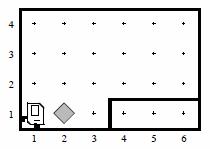
\includegraphics[scale=0.80]{karel_the_robot}
	\caption[Karel the Robot]{A simple \emph{Karel the Robot} level, where Karel (bottom left) must move to and pick up a single beeper (diamond shape). \emph{Image source:~\cite{roberts:karel_the_robot_java}}}
	\label{fig:karel_the_robot}
\end{figure}

\noindent
Karel the Robot has now been around for more than 30 years, and the teaching paradigm described has proved successful in introducing students to the art of programming.\footnote{See for example~\cite{krause:computer_science_air_force},~\cite{untch:karel_conventional_language},~\cite{becker:teaching_with_karel}} Students are allowed to explore advanced concepts in a safe environment with less relevant complexities removed, and in a way that makes them \emph{want} to learn. The concept has been adapted and refined in many ways over the years, but the core paradigm remains.

\subsection{Josef the Robot}
\label{sec:josef_the_robot}
Josef the Robot~\cite{tomek:josef_the_robot} is a game-like programming environment similar to Karel (Sect.~\ref{sec:karel_the_robot}). Unlike Karel, Josef more closely resembles ``real'' programming languages by being rich in structures and operations. Like Karel, Josef is also inspired by the LOGO project.

\noindent
The author of Josef, Ivan Tomek, provides ample motivation for creating a more novice-friendly environment for learning how to program. Firstly, potential learners should find the problems they can solve with programming to be interesting, which is likely not the case (for the average person) with problems like sorting a sequence of numbers. Furthermore, novice programmers should not have to worry about the more complex rules that are not directly related to problem-solving, such as syntax and data handling.

\subsection{Serious and Epistemic Games}
\label{sec:serious_games}
Games that are designed for a purpose that is not pure entertainment are often called \emph{Serious Games}, a term likely popularized by \emph{The Serious Games Initiative}\footnote{\url{http://www.seriousgames.org/}} in 2002~\cite{djaouti:serious_games_origins}. This genre encompasses many different types of games, but a prime example of a serious game is the \emph{flight simulator}, a realistic type of game that exists in various forms, and is extensively used to teach pilots how to fly aircraft.

\noindent
The idea behind serious games is to improve student motivation and engagement by providing immersive learning experiences, similar to how many professions are taught. I can read a lot about woodworking, but in order to become a good carpenter, I must practice. Seeing actual results of my knowledge and skills in woodworking is also likely to be more enjoyable than simply imagining how it might look. Games can provide a similar kind of (simulated) hands-on experience for topics that are difficult or inconvenient to practice immersively, especially more abstract topics like math or computer programming, and this has also proved to be a more efficient learning method in many cases. Children especially learn and are better motivated by the kind of problem-solving we find in games, as opposed to traditional textbook learning~\cite{freitas:serious_games_new_paradigm}.

\noindent
Several organizations working with serious games exist. Some examples are the \emph{Serious Games Institute},\footnote{\url{http://www.seriousgamesinstitute.co.uk/}} the \emph{Games Learning Society},\footnote{\url{http://www.gameslearningsociety.org/}} the \emph{Learning Games Network},\footnote{\url{http://learninggamesnetwork.org/}} and \emph{Serious Games Interactive}.\footnote{\url{http://www.seriousgames.net/}} These represent both commercial, societal, and academic interest in serious games.

\noindent
Researchers at the University of Wisconsin coined the term \emph{Epistemic Games} for the subset of serious games that aim to teach specific professions or skills~\cite{shaffer:epistemic_games}. They argue that games can help teach students to apply their knowledge, instead of simply remembering, in addition to facilitate for \emph{innovative} learning. With this as a basis, \emph{The Games and Professional Simulations Research Consortium}\footnote{\url{http://edgaps.org/gaps/}} has been formed in order to solve educational challenges through games and simulations.

\subsection{CodeSpells}
\label{sec:codespells}
\emph{CodeSpells} is a project from the University of California, San Diego, that aims to teach Java programming through a wizardry game~\cite{esper:codespells}. The CodeSpells team draws inspiration from the \emph{epistemic games} concept, and their games immerses novice programmers in a world that connects abstract code (Fig.~\ref{fig:codespells_spell}) with visual and ``physical'' effects in the environment (Fig.~\ref{fig:codespells_fire}).

\begin{figure}[htp]
	\centering
	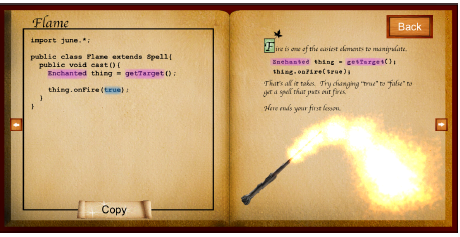
\includegraphics[scale=0.80]{codespells_spell}
	\caption[Java code for a CodeSpells spell]{An example of the CodeSpells spellbook, with Java code for the \emph{Flame} spell. The second page adds a short description, and a tip on how the spell can be modified. \emph{Image source:~\cite{esper:codespells}}}
	\label{fig:codespells_spell}
\end{figure}

\begin{figure}[htp]
	\centering
	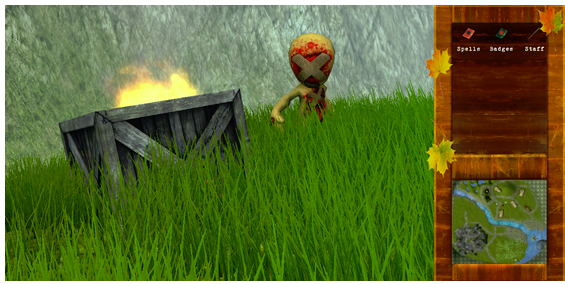
\includegraphics[scale=0.80]{codespells_fire}
	\caption[The CodeSpells game environment]{The game environment presented to the user in \emph{CodeSpells}. In this particular quest, the player must modify the \emph{Flame} spell (Fig.~\ref{fig:codespells_spell}) in order to extinguish the fire by setting \emph{thing.onFire(false)}. Image source: \emph{\url{https://sites.google.com/a/eng.ucsd.edu/codespells/home/level-1-quests}}}
	\label{fig:codespells_fire}
\end{figure}

\noindent
An important goal for the CodeSpells project is for students to gain a deep understanding of the programming language they use and problems they solve, and retain this understanding after completing the game. They would also like the students to be able to play the game without instructor assistance, and have focused extensively on designing quests that provide the appropriate scaffolding, as well as encourage exploration beyond the minimum required to move on~\cite{esper:design_quests_java_concepts}.

\noindent
In order to verify and improve the usefulness of their game for teaching programming, the CodeSpells team have conducted some user studies. Through these studies, they discovered that by immersing users in the game, the users developed a determination and a positive outlook on solving programming challenges~\cite{esper:codespells}. The team also discovered some principles that can be used to improve quest design~\cite{esper:design_quests_java_concepts}:

\begin{itemize}
	\item Provide examples that can be tested and used as a starting point, allowing users to see their effects.
	\item While the introduction should make it possible to perform complex actions with little effort, expectations for more effort should be provided from the beginning, letting users know that they have to build on and modify the examples.
	\item Provide directed exploration through quests, so the user can get a sense of complexity ordering and a choice of which challenge to overcome.
\end{itemize}

\noindent
These principles can likely also be used to improve design of other serious games.

\subsection{Non-Serious Games}
\label{sec:non-serious_games}
While the term \emph{Serious Games} covers the type of games that are designed for purposes other than entertainment, there are many examples of games designed for entertainment that ``accidentally'' teach their players valuable skills and knowledge.

\noindent
James P. Gee is a famous advocate for game-based learning. Through his analysis of various ``non-serious'' games, he identifies good principles of learning present in many of these games~\cite{gee:learning_machines}:

\begin{itemize}
	\item{\textbf{Empowered Learners:}} Players feel like active agents while playing, and not just passive recipients of information. Games are interactive, which leads to perceived ownership and engaged participation.
	\item{\textbf{Customization:}} Players are in many cases allowed to make choices about how to play, such as adjusting difficulty or playing style. People are different, and learn in different ways.
	\item{\textbf{Identity:}} Players often take on new identities within the game, in which they become heavily invested. This leads to a level of commitment that facilitates for deep learning.
	\item{\textbf{Manipulation and Distributed Knowledge:}} When players are able to control and manipulate a character or an object in the game environment, they feel expanded and empowered. Often, part of the knowledge required for manipulation is stored in the game itself (automated), so that the player can focus on the parts that are important for their task (and ``level of abstraction'').
	\item{\textbf{Well-ordered Problems:}} Players are exposed to problems in a well-ordered manner, so that they can form hypotheses that not only work in the moment, but prepare them for more difficult challenges later in the game.
	\item{\textbf{Pleasant Frustration:}} Players are exposed to problems that are neither too easy or too hard, but at the edge of the players' competence, and at their own pace.
	\item{\textbf{Cycles of Expertise:}} Players are allowed to repeat and practice skills until they become nearly automatic. Then, as the game progresses, they might have to adapt their skills to new conditions, and repeat the cycle.
	\item{\textbf{Context-sensitivity of Information:}} Players are often presented with the information they need \emph{when} they need it, instead of having to memorize it in advance.
	\item{\textbf{Fish Tanks:}} In many cases, games serve as simplified versions of real-world systems, and illustrate some important concepts while hiding complexities that might be too difficult to handle for novices. Sometimes, such fish tanks are also created within the game itself, in the form of tutorials. This allows players to exercise their skills without having to worry about \emph{all} the details.
	\item{\textbf{Sandboxes:}} Games also provide a safe environment for exercising skills, where the cost of failure generally is low compared to the real world.
	\item{\textbf{Skills as Strategies:}} Instead of practicing for the sole purpose of becoming good, players see the skills they learn as a strategy towards accomplishing goals within the game. This provides better motivation by allowing ``in-context'' practice.
	\item{\textbf{System Thinking:}} Many games consist of smaller elements, where players must understand how all the elements interact fit into the overall system of the game.
	\item{\textbf{Meaning as Action Image:}} Instead of just providing definitions and descriptions, games present concepts through visualizations and experiences, which is closer to how people actually think.
\end{itemize}

\noindent
These are clearly principles that should be considered also in serious and educational games, not only those made for entertainment. As Gee points out, \emph{``When we think of games, we think of fun. When we think of learning, we think of work''}. If done right, it is likely possible to merge the tedious process of learning with the fun of games with equal or better results.

\subsection{A Summary of Good Practices for Educational Games}
\label{sec:good_practices_games}
While educational games by default generally incorporate some good learning practices (interactivity and feedback), some ways of designing and implementing such a game are likely better than other. Based on the work described in the previous sections as well as Sect.~\ref{sec:game_based_learning}, this section summarizes some additional aspects that should be considered when designing an educational game.

\paragraph{Tutorials} Many games start by guiding the player through a tutorial in order to learn the basics of the game, which is similar to completing a tutorial in order to learn about a topic like programming language. Games, particularly complex ones, may benefit from having a tutorial introduction, in the form of increased player engagement~\cite{andersen:tutorials_impact}. Since educational games are often used to teach complex concepts, creating a tutorial is generally justified. The principles listed in Sect.~\ref{sec:good_practices_tutorials} also apply to tutorials for educational games, since these should be at least as good as tutorials for teaching a specific topic. Because of their immersive nature, video games likely makes a some of these principles easier to follow, such as providing good visual mapping of \gls{ui} elements and suitable multimedia content.

\paragraph{Immersion} By providing an \emph{immersive} experience, educational games can provide better motivation and encouragement for players to interact with and explore the concepts taught~\cite{esper:codespells}. Providing an immersive experience may include giving the player a sense of \emph{identity} in the game, enhancing commitment, or provide \emph{fish tanks} or \emph{sandboxes} where players can discover, explore, and experiment with concepts in safe and possibly simplified environments~\cite{gee:learning_machines}. Immersive game experiences also provide players with meaning for verbal concepts, through visualizations and experiences~\cite{gee:learning_machines}.

\paragraph{Exploration and Guidance} The discussion of exploration versus guidance becomes even more important for educational games than for tutorials. Good educational games often provide a safe environment where concepts can be explored and experimented with, even without any guidance. In many cases, too much guidance may even prevent exploration and discovery to some degree~\cite{bonawitz:double_edged_pedagogy}. Depending on the complexity of the concepts taught, having no guidance at all is also not a good solution. Some players will have more trouble than others understanding certain concepts, and subtleties are not always intuitively understood. The optimal solution is to evaluate the game's complexity, and provide some kind of middle ground (directed exploration,~\cite{esper:design_quests_java_concepts}) tailored not only to how difficult the concepts are, but the player's previous knowledge and ability to understand them. Users may even be allowed to choose their own difficulty level based on their own perceived experience level and skill.

\paragraph{Simplicity and Challenge} Irrespective of their background, any users within the target audience should be able to get started and see results early in the introduction~\cite{esper:design_quests_java_concepts}. However, the problems presented must eventually become difficult enough to allow players to gain deep understanding of the concepts taught, and expectations of this should be present from the beginning. Additionally, players can progressively be presented with an environment that is more and more like a real environment. This can help make the transition from practicing skills in a video game, to using these skills in real situations smoother~\cite{untch:karel_conventional_language}.

\cleardoublepage
\chapter{Discussion and Conclusion}
\label{ch:discussion}
The work of this thesis has been focused around creating a better environment for learning about software modeling languages, more specifically focusing on \gls{uml} activities within the context of the \emph{Reactive Blocks} modeling tool. Inspired primarily by methods used to teach players how to play video games, two different learning environments were explored.

\section{The Tutorial}
\label{sec:discussion_tutorial}
The first teaching method explored was the \emph{tutorial}, a concept widely used to teach various topics by offering interactive introductions, often with exercises. This approach to teaching is also used in many video games, where players are exposed to a tutorial that teaches them the basics of the game before they are allowed to explore the game on their own. The design, implementation, testing, and evaluation of the tutorial is covered in Ch.~\ref{ch:reactive_blocks_tutorial}.

\noindent
When creating the tutorial, various learning practices were taken into consideration. These were a mixture of good practices for video game tutorials and other types of tutorials, from both formal and informal sources. A summary of these is provided in Sect.~\ref{sec:good_practices_tutorials}.

\noindent
A few iterations of going through \gls{uml} activity concepts and figuring out their interdependencies, finding the least amount of information required to describe them accurately, and designing suitable exercises for understanding their semantics, resulted in a seven-step tutorial. Each step gave a short introduction of one or more concepts, and challenged learners with an exercise to solve using these concepts. The tutorial and its seven steps is described in more detail in Sect.~\ref{sec:tutorial_design}.

\noindent
Unfortunately, not all of these practices were feasible to implement within the given frame, particularly because of the constrains provided by the proprietary Reactive Blocks modeling environment. This meant some of the goals that had initially been set for the tutorial had to be forgone, and some adjustments had to be made to the tutorial design. The most prominent change was that all concept and task information had to be provided outside the modeling environment, in a supplementary document. Sections~\ref{sec:tutorial_goals_fulfilled} and~\ref{sec:tutorial_goals_not_fulfilled} provide a more detailed overview of the extent to which each goal was fulfilled by the tutorial design and implementation.

\noindent
In order to uncover any major flaws or issues with the tutorial, and additionally get an impression of its teaching potential, a user test with a small number of test subjects was conducted. The testing session revealed a number of issues that required some additional consideration, and the main bulk of these were related, directly or indirectly, to the use of Reactive Blocks as the modeling environment. The session also provided some indications that the tutorial could indeed be a very good way of learning about \gls{uml} activities, particularly with respect to providing motivation for learners. The tutorial may not be an adequate tool for learning to use Reactive Blocks however, as follow-up observations of the test subjects revealed that many of them struggled when working with Reactive Blocks, on account of the concepts that were not covered in the tutorial.

\noindent
Although I was unable to implement and test several of the tutorial design principles, the tutorial served as a good starting point for establishing a teaching order for concepts in \gls{uml} activities, and figuring out how much information users need in order to solve certain types of exercises related to each concept. These results laid the foundation for the \emph{Reactive Blocks game}, which was the second teaching method explored.

\section{The Game}
\label{sec:discussion_game}
The second teaching method explored in this thesis was to teach \gls{uml} activity concepts inside a game. Learning games are becoming very popular in many levels of education because they offer a more immersive and interactive learning experience, among other things. Teaching \gls{uml} activities with a game gave more potential for utilizing game strategies for introducing and teaching new concepts, such as giving learners a sense of \emph{empowerment} and \emph{identity}. The design, implementation, testing, and evaluation of the learning game is covered in Ch.~\ref{ch:tutorial_game}.

\noindent
Like with the tutorial, the learning game is based on a set of principles for designing this type of game, and these are summarized in Sect.~\ref{sec:good_practices_games}. Additionally, the game would have a lot in common with a tutorial, so consideration was made with respect to the principles for good tutorials, and the lessons learned from the design and testing of the tutorial in Ch.~\ref{ch:reactive_blocks_tutorial}.

\noindent
The design and implementation process resulted in a first prototype version of a game with 5 levels, covering only part of the seven steps from the tutorial. The game was meant to have more levels, but we wanted to conduct a usability study in order to discover any serious issues as early as possible. The concept of the game is a two-dimensional world, where the player controls a character, performing various tasks. The character is controlled entirely through \gls{uml} activity/Reactive Blocks models, which the player has to set up prior to launching the game level. Each level also has an introduction part, similar to the introductions given with the tutorial, but more extensive and with additional resources. The complete design and implementation of the game is covered in Sections~\ref{sec:game_design} and~\ref{sec:game_implementation}.

\noindent
While the game format allowed consideration and implementation of some additional ``good'' practices, there were still issues that were difficult to deal with because of the Reactive Blocks modeling environment. A usability test with three test subjects revealed that all three, who were novice users, had difficulties with correctly understanding and using a number of \gls{ui} processes and elements in Reactive Blocks. This was despite the fact that some additional \gls{ui} help had been added to the introduction part of the game, as a result of some of the same issues appearing in the tutorial test. Apart from those related to Reactive Blocks, the usability test revealed only minor \gls{ui} issues that could be taken into consideration for the next version of the prototype.

\noindent
In addition to usability-related results, the testing sessions also revealed that the test subjects gained a lower understanding of the concepts presented than desired. Some hints of potential misconceptions were also observed. This could likely mean that 5 levels is not sufficient to really learn these concepts, and that more practice is required. If this is the case, it can be solved by adding additional levels and challenges, for the players to practice their skills and knowledge more, and with different perspectives. In any case, more testing is needed to properly verify and understand the issue, preferably on a more complete version of the game.

\noindent
On a brighter note, all three subjects stated that they enjoyed the game as a tool for learning about \gls{uml} activities and Reactive Blocks, and would likely prefer it over other ways of learning. However, more than three opinions are likely needed in order to verify a real interest in this type of learning resource. It also remains to be seen whether a game like this will instill deep learning in players, but research supports that this is the case for well-designed educational games (see Sect.~\ref{sec:game_based_learning}).

\noindent
The game is still in a relatively early stage, but the results so far are encouraging. Further development of the game will however not continue within the scope of this thesis, because of time constraints.


\section{Concluding Remarks}
\label{sec:concluding_remarks}
The work of this thesis has been about exploring the use of game-related learning principles and strategies for teaching software modeling with \gls{uml} activities. Two different teaching approaches were explored:  the first approach simply incorporated many of the learning principles in a stepwise modeling tutorial, and the second approach involved designing a game with levels teaching the same steps, but in a more immersive environment.

\noindent
Some minor tests of the two approaches were conducted, yielding indicative but interesting results. Both approaches were found to be flawed in some ways, but they also showed great potential for teaching the concepts in question to the target audience in an interesting and motivating way. It is however difficult to draw any conclusions about how the two approaches would measure up against other learning resources for the same concepts, without data from comparative studies.

\noindent
It is also worth noting that with regard to established theoretical usability and learning principles, both approaches measure up quite well by \emph{design}, despite the \emph{implementations} lacking some important features. Whether implementing all of these features will actually be beneficial to the learning experience or not is however a little uncertain, as users have been known to behave unpredictably~\cite{andersen:tutorials_impact}.

\noindent
In the end, there is no reason to believe that learning strategies from games will \emph{not} be appropriate also for learning modeling languages, as there have been no results indicating this. At the same time, there is not enough ground in this thesis alone to conclude that they \emph{definitely will be} appropriate either. There are however several other research efforts endorsing this approach for teaching programming, which is a very closely related topic.

\noindent
The conclusion to be drawn from this thesis is the following: using learning strategies from games to teach modeling languages is definitely worth exploring, but designing and implementing a good learning environment is not trivial, and requires a considerable amount of work and effort. Hopefully, the work and examples provided here can serve as a starting point for others.

\clearpage

\section{Future Work}
\label{sec:future_work}
As the final part of this thesis, some suggestions for future work are included. There are several possible paths to take, and some are described in the following sections.

\subsection{Complete Game}
The most prominent path to take would be to continue development of the Reactive Blocks game, improving on the prototype and moving closer to a ``finished'' game. The current prototype is a little lacking in content, in addition to needing some minor fixing. There is also great potential for improving the modeling environment, particularly in order to improve usability. Section.~\ref{sec:game_improvement} contains some more concrete suggestions on how to continue the development of the game. 

\subsection{Comparative Studies}
The weakest part of this thesis is likely that I was unable to perform proper comparative studies, pitting the \emph{Reactive Blocks game} against other similar learning resources in order to measure factors like player engagement and levels of understanding. This was not feasible because of constraints on time and resources. Comparative studies would however have been prudent in this context, and should thus be the second priority for any future work (after fixing the simpler issues and adding more content to the game).

\noindent
More specifically, the game can be studied in comparison to the tutorial in Ch.~\ref{ch:reactive_blocks_tutorial}, any of the existing tutorials mentioned in Sect.~\ref{sec:existing_tutorials}, or the lazier approach of just letting learners dig through documentation.

\subsection{Other Modeling Languages}
This thesis has been focused around teaching \gls{uml} activities, more specifically in the context of Reactive Blocks, using teaching principles and strategies from games. It could also be interesting to use the same approach with other modeling languages, such as \gls{uml} state machines, sequence diagrams, flowcharts, or even class diagrams. These will likely provide different challenges with respect to game and exercise design, but allow use of the same teaching principles.
\cleardoublepage

\renewcommand*{\bibname}{References}
\bibliographystyle{alpha}
\bibliography{main}

%% Uncomment the following if you have any appendix
\appendix
\addtocontents{toc}{%
 \protect\vspace{1em}% 
 \protect\noindent \bfseries \appendixtocname\protect\par
 \protect\vspace{-.5em}%
}
\renewcommand{\chaptername}{\appendixname}
%% include below possible appendices (chapters)
\begin{appendices}

\chapter{UML Activities Tutorial}
\label{appx:tutorial}
The following pages contain the complete document for the Reactive Blocks \gls{uml} Activities tutorial described in Ch.~\ref{ch:reactive_blocks_tutorial}.
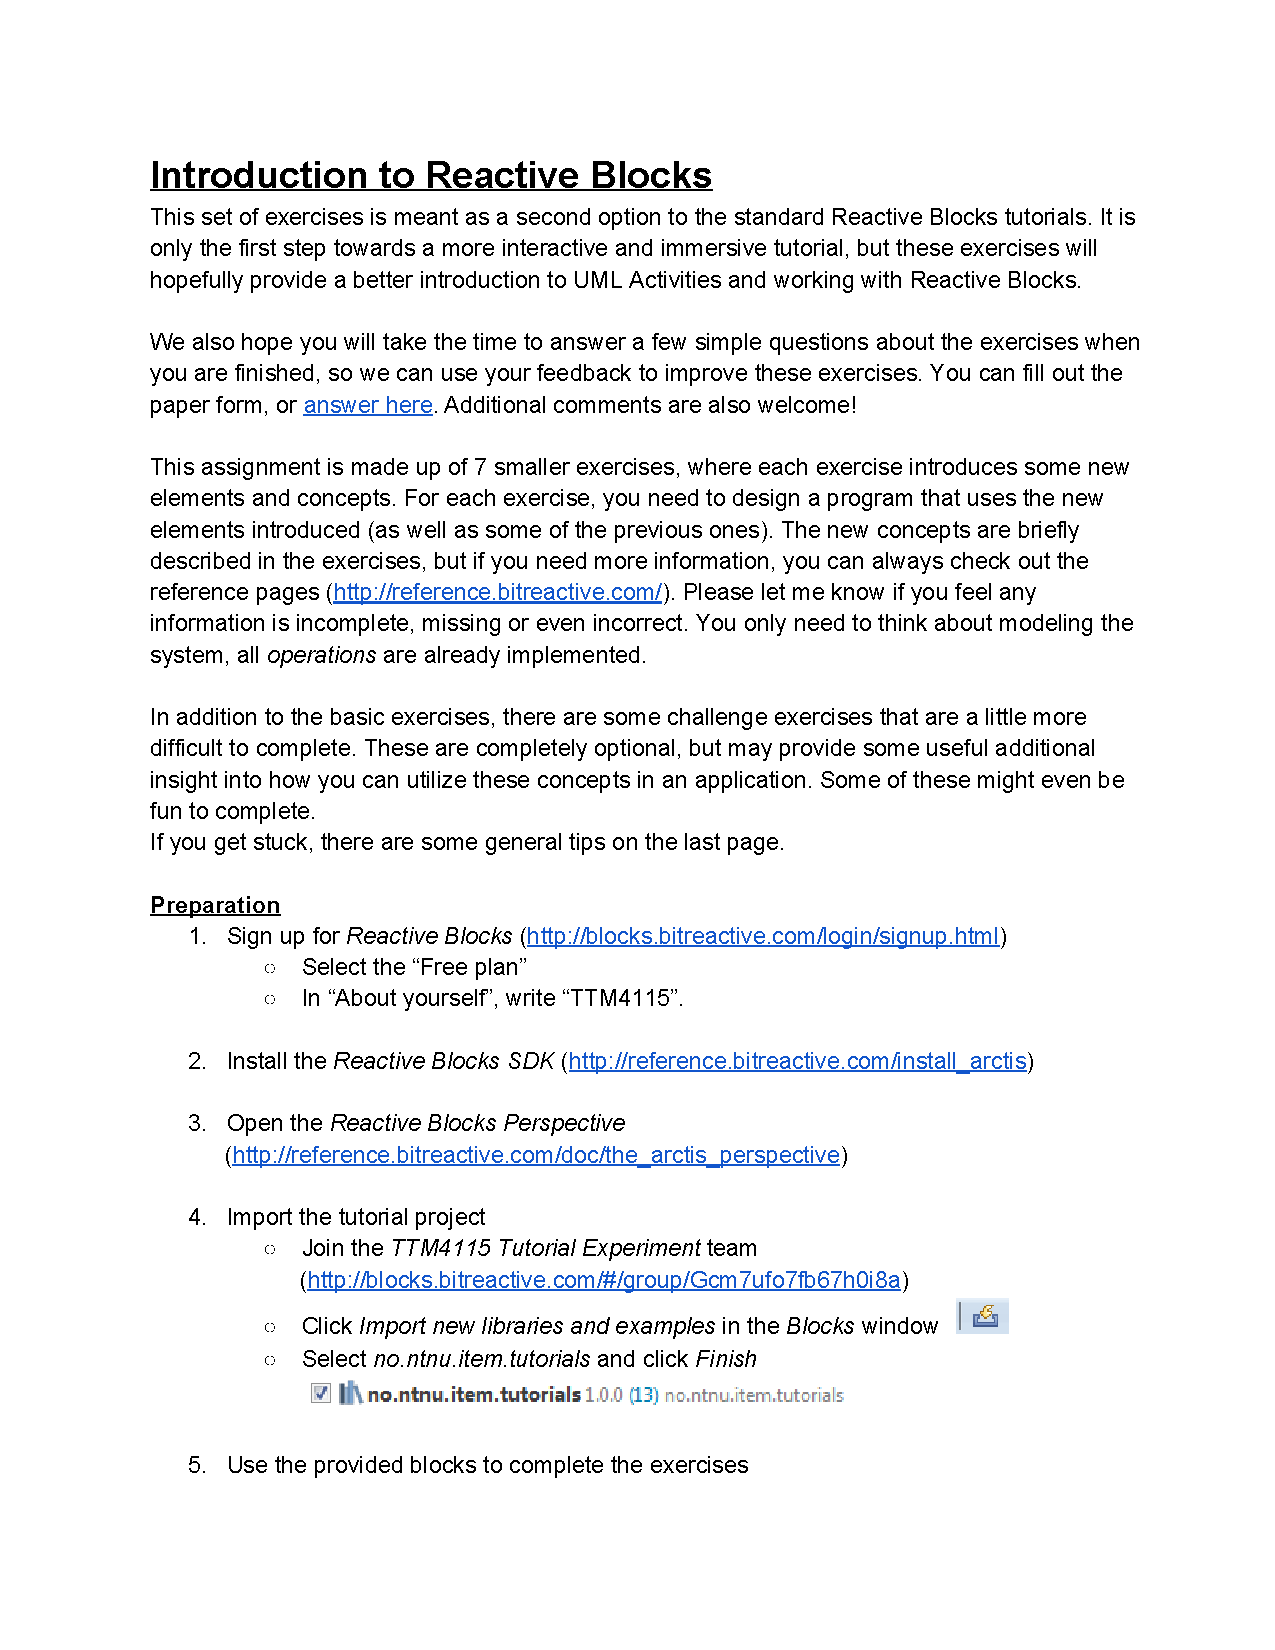
\includepdf[pages={-}]{tutorial_exercises.pdf}

\chapter{Tutorial Feedback Form}
\label{appx:feedback_form}

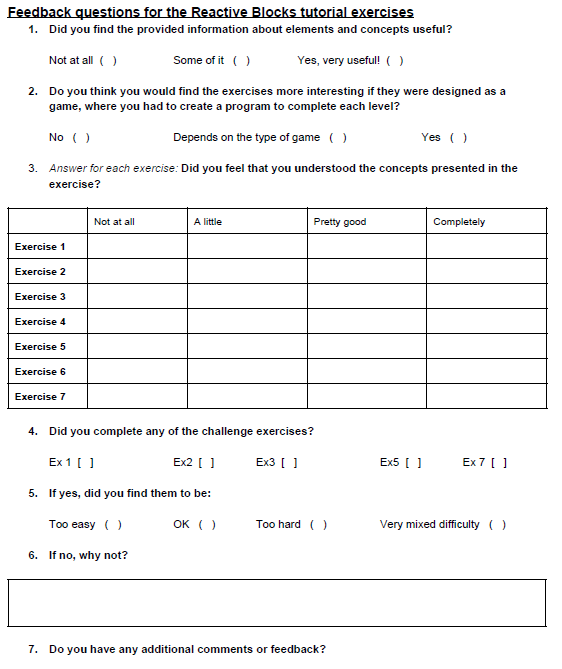
\includegraphics[scale=0.75]{tutorial_feedback}

\chapter{Tutorial User Test Data}
\label{appx:tutorial_test_data}
This section contains all the data gathered with the feedback forms (Appx.~\ref{appx:feedback_form}) in the user test for the Reactive Blocks/\gls{uml} Activities tutorial (Ch.~\ref{ch:reactive_blocks_tutorial}).

\begin{figure}[htp]
	\centering
	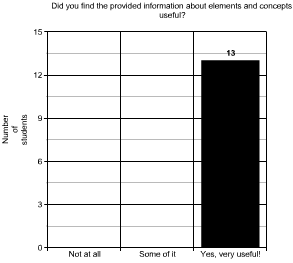
\includegraphics[scale=0.80]{feedback_form_q1}
	\caption[Results from feedback form question 1]{Results from question 1 of the feedback form (Appx.~\ref{appx:feedback_form}). The total number of students was 13.}
	\label{fig:feedback_form_q1}
\end{figure}

\begin{figure}[htp]
	\centering
	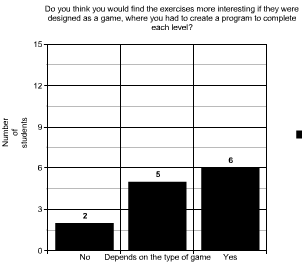
\includegraphics[scale=0.80]{feedback_form_q2}
	\caption[Results from feedback form question 2]{Results from question 2 of the feedback form (Appx.~\ref{appx:feedback_form}). The total number of students was 13.}
	\label{fig:feedback_form_q2}
\end{figure}

\begin{figure}[htp]
	\centering
	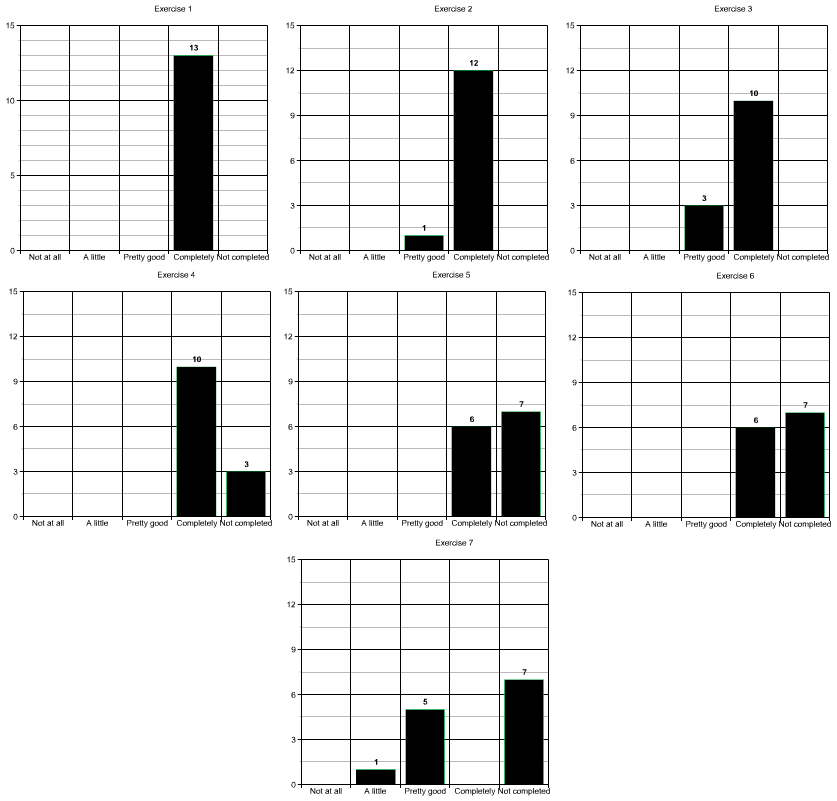
\includegraphics[scale=0.55]{feedback_form_q3}
	\caption[Results from feedback form question 3]{Results per exercise from question 3 of the feedback form (Appx.~\ref{appx:feedback_form}). The value on the y-axis for all graphs is the number of students who chose that answer. The total number of students was 13.}
	\label{fig:feedback_form_q3}
\end{figure}

\begin{figure}[htp]
	\centering
	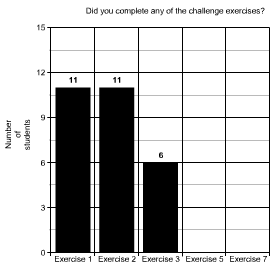
\includegraphics[scale=0.80]{feedback_form_q4}
	\caption[Results from feedback form question 4]{Results from question 4 of the feedback form (Appx.~\ref{appx:feedback_form}). The total number of students was 13.}
	\label{fig:feedback_form_q4}
\end{figure}

\begin{figure}[htp]
	\centering
	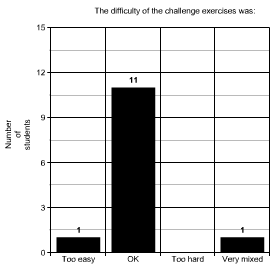
\includegraphics[scale=0.80]{feedback_form_q5}
	\caption[Results from feedback form question 5]{Results from question 5 of the feedback form (Appx.~\ref{appx:feedback_form}). The total number of students was 13.}
	\label{fig:feedback_form_q5}
\end{figure}

\chapter{Feedback Form for the Game Usability Test}
\label{appx:game_feedback_form}

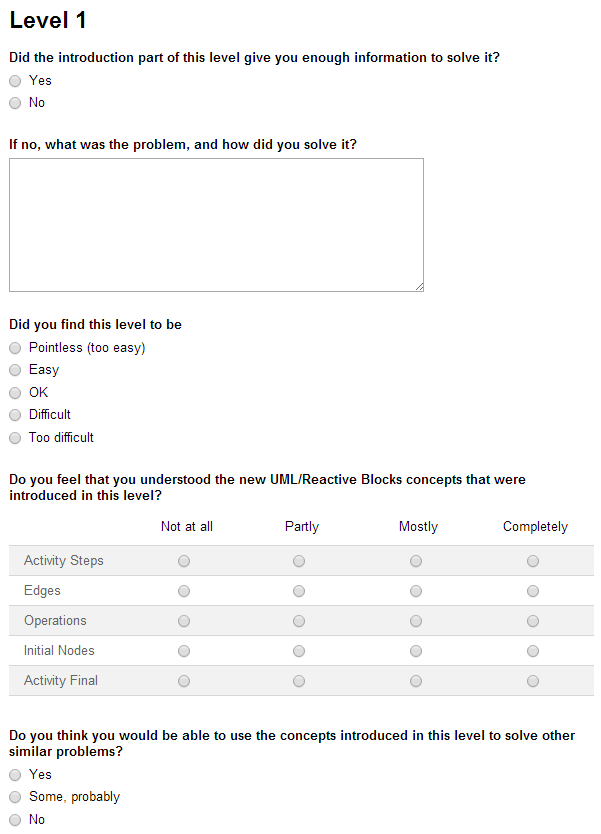
\includegraphics[scale=0.60]{usability_quiz}







\end{appendices}


\end{document} 
